%!TEX root = ../Thesis.tex
\begin{figure}[ht]
  \centering
  \begin{subfigure}[b]{0.45\textwidth}
    \centering
    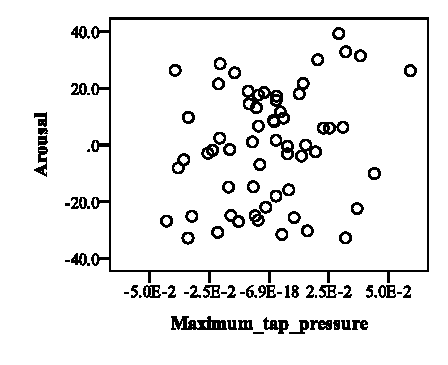
\includegraphics[width=\textwidth]{images/linearity/partialregression/arousal/ArMaxMax.eps}
    \label{fig:armaxmax}
  \end{subfigure}
  \quad
  \begin{subfigure}[b]{0.45\textwidth}
    \centering
    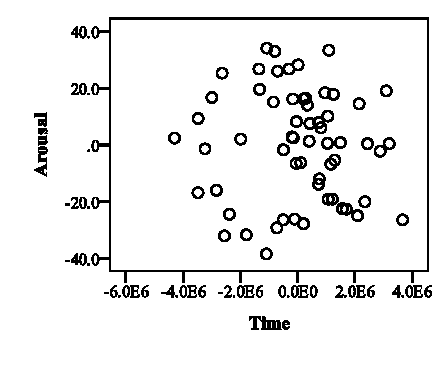
\includegraphics[width=\textwidth]{images/linearity/partialregression/arousal/ArMaxTime.eps}
    \label{fig:armaxtime}
  \end{subfigure}
  \caption{Partial regression plots with arousal (dependent variable), maximum pressure and duration (independent variables). Note the approximate linearity.}
\end{figure}

\begin{figure}[ht]
  \centering
  \begin{subfigure}[b]{0.45\textwidth}
    \centering
    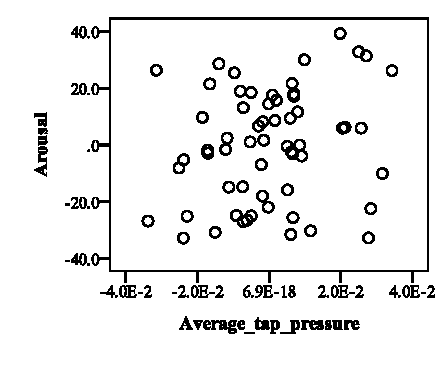
\includegraphics[width=\textwidth]{images/linearity/partialregression/arousal/ArAvgAvg.eps}
    \label{fig:aravgavg}
  \end{subfigure}
  \quad
  \begin{subfigure}[b]{0.45\textwidth}
    \centering
    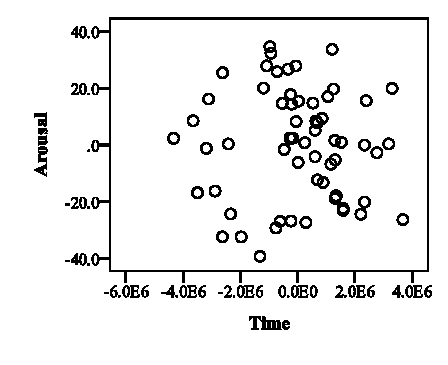
\includegraphics[width=\textwidth]{images/linearity/partialregression/arousal/ArAvgTime.eps}
    \label{fig:aravgtime}
  \end{subfigure}
  \caption{Partial regression plots with arousal (dependent variable), average pressure and duration (independent variables). Note the approximate linearity.}
\end{figure}